\documentclass[a4paper,12pt]{article}
\usepackage[spanish]{babel}
\usepackage[utf8]{inputenc}
\usepackage{amsmath}
\usepackage{enumitem}
\usepackage{hyperref}
\usepackage{geometry}
\usepackage{fancyhdr}
\usepackage{graphicx}
\usepackage{color}
\geometry{margin=2.5cm}
\pagestyle{fancy}
\fancyhf{}
\rhead{Jesús Losada Arauzo}
\lhead{Práctica6}
\rfoot{\thepage}

\title{\textbf{Práctica6} \\ \large Sistema experto con razonamiento basado en certeza}
\author{Jesús Losada Arauzo\\ DNI: 77201609Q}
\date{23 de mayo de 2025}

\begin{document}
\maketitle
%\tableofcontents
\newpage

\section{Resumen del funcionamiento del sistema}
El sistema implementado es un sistema experto en CLIPS cuyo objetivo es seleccionar una receta y razonar si le gustará o no a un grupo específico de personas ---en este caso, los niños--- utilizando razonamiento con \textbf{factores de certeza}. Para ello, tras elegir una receta según criterios definidos, se analiza su composición y características (dulzura, si es postre, picante, con verdura, etc.), y a través de reglas con certeza, se deduce si es probable que guste a los niños.

\section{Descripción del proceso seguido}

\subsection{Procedimiento seguido para el desarrollo de la base de conocimiento}
La base de conocimiento se construyó inicialmente con hechos básicos sobre recetas, ingredientes y propiedades como: si es vegetariana, contiene verdura, si es postre, etc. Posteriormente, se añadieron módulos con reglas de inferencia que permiten deducir propiedades o seleccionar una receta.

En una segunda fase, se ha ampliado la base de conocimiento con un \textbf{módulo de certeza}, que permite razonar a partir de evidencias con valores numéricos en el intervalo $[-1, 1]$, acumulando y combinando el impacto de distintas evidencias.

\subsection{Procedimiento de validación y verificación del sistema}
El sistema ha sido validado introduciendo recetas con ingredientes variados (verdura, carne, dulces...) y observando si las inferencias con certeza se realizan correctamente. Se ha verificado que:

\begin{itemize}
  \item Se activa el módulo de certeza al elegir una receta.
  \item Se generan las evidencias correctamente.
  \item Las reglas modifican la certeza acumulada correctamente.
  \item Se muestra una conclusión clara y justificada.
\end{itemize}

\section{Descripción del sistema}

\subsection{Variables de entrada}
Las variables de entrada del módulo de certeza son:
\begin{itemize}
  \item \textbf{tiene\_verdura}
  \item \textbf{tiene\_carne}
  \item \textbf{tiene\_dulce}
  \item \textbf{es\_picante}
  \item \textbf{es\_postre}
\end{itemize}

Estas se deducen de los hechos sobre ingredientes y propiedades de la receta seleccionada.

\subsection{Variable de salida}
La variable de salida principal es:
\begin{itemize}
  \item \textbf{Certeza de que gustará a los niños (ninios)}
\end{itemize}

\subsection{Conocimiento global del sistema}
El sistema carga hechos como:
\begin{itemize}
  \item \texttt{(receta (nombre ...) (tipo\_plato ...))}
  \item \texttt{(es\_un\_ingrediente\_de ...)}
  \item \texttt{(es\_un\_tipo\_de ...)}
  \item \texttt{(propiedad\_receta ...)}
\end{itemize}

Y utiliza plantillas para representar justificaciones y factores de certeza.

\subsection{Estructura en módulos}
\begin{itemize}
  \item \textbf{Módulo principal de elección de receta}
  \item \textbf{Módulo de certeza: calcular\_certeza\_gustar\_a\_ninios}
\end{itemize}

\subsubsection{Descripción del módulo de certeza}
\textbf{Objetivo:} Calcular si una receta gustará a los niños basándose en ciertas propiedades.  
\textbf{Conocimiento que utiliza:} Evidencias como "tiene\_dulce" o "es\_picante", y reglas con factores de certeza.  
\textbf{Conocimiento que deduce:} La certeza final y una justificación textual.

\subsubsection{Hechos y reglas del módulo de certeza}
\begin{itemize}
  \item Hechos: \texttt{Evidencia}, \texttt{FactorCerteza}, \texttt{justificacion\_certeza}
  \item Reglas:
  \begin{itemize}
    \item \texttt{certeza\_evidencias}: convierte evidencias en certeza inicial.
    \item \texttt{R1}–\texttt{R5}: ajustan la certeza según la propiedad.
    \item \texttt{combinar}: gestiona combinaciones de factores por múltiples caminos.
    \item \texttt{fin\_certeza}: concluye el proceso y da explicación textual.
  \end{itemize}
\end{itemize}

\section{Breve manual de uso del sistema}
\begin{enumerate}
  \item Cargar el sistema en CLIPS con \texttt{(load "Practica6.clp")}
  \item Inicializar con \texttt{(reset)}
  \item Ejecutar con \texttt{(run)}
  \item Se mostrará la receta elegida y su justificación.
  \item Si hay activación del módulo de certeza, también se mostrará si gustará a los niños y por qué.
\end{enumerate}

\section*{Ejemplo de ejecución}
\begin{figure}[h!]
    \centering
    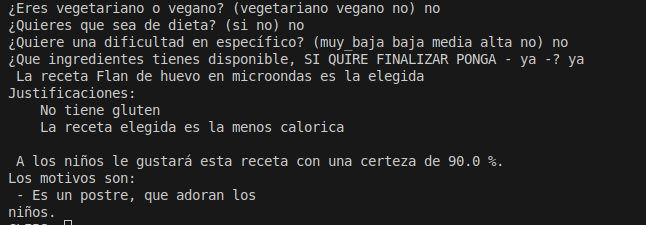
\includegraphics[width=0.9\textwidth]{captura1.png}
    \caption{Salida del sistema con una receta elegida y cálculo de certeza}
\end{figure}


\end{document}

